%
% File acl2014.tex
%
% Contact: g.colavizza@uva.nl
%%
%% Based on the style files for ACL-2013, which were, in turn,
%% Based on the style files for ACL-2012, which were, in turn,
%% based on the style files for ACL-2011, which were, in turn, 
%% based on the style files for ACL-2010, which were, in turn, 
%% based on the style files for ACL-IJCNLP-2009, which were, in turn,
%% based on the style files for EACL-2009 and IJCNLP-2008...

%% Based on the style files for EACL 2006 by 
%%e.agirre@ehu.es or Sergi.Balari@uab.es
%% and that of ACL 08 by Joakim Nivre and Noah Smith

\documentclass[11pt]{article}
\usepackage{acl2014}
\usepackage{times}
\usepackage{url}
\usepackage[hyphens]{url}
\usepackage{latexsym}
\usepackage{graphicx}

%\setlength\titlebox{5cm}

% You can expand the titlebox if you need extra space
% to show all the authors. Please do not make the titlebox
% smaller than 5cm (the original size); we will check this
% in the camera-ready version and ask you to change it back.


\title{The Bell Jar through Python magnifying glass}

\author{Martina Biagioni \\
  {\tt martina.biagioni2@studio.unibo.it} }

\date{15710/2024}

\begin{document}
\maketitle
\begin{abstract}
"The Bell Jar" by Sylvia Plath is a classic American coming of age novel. Set in the 1950s, it shows an America shaped by conservative values and a patriarchic structures, a society that places women under particular restraints. The ideals of purity, chastity, the aspiration to live as suburban mother and homemaker, rather than pursuing their own career, weighed heavily on Plath, and these themes resonate throughout the book.
The goal of this project is to analyze the novel computationally using Python and compare insights from computational methods to traditional human analysis.

\end{abstract}


\section{1. Introduction}
"The Bell Jar" portrays the author’s character and her struggles with mental health. This coming of age novel shows growth trough pain and rebirth: Esther, the main character, doesn't experience life-changing events as something positive, but as a regression into madness, that will culminate in a suicide attempt. 
Her first time in New York City, her first marriage proposal, her successes in college are upsetting and disorienting to her. Her struggles and triumphs seem more heroic than conventional achievements. In fact, her desire to die rather than live a false life can be interpreted as noble, and the gradual steps she takes back to sanity seem dignified. Esther does not mark maturity in the traditional way of fictional heroines, by marrying and beginning a family, but by finding the strength to reject the conventional model of womanhood. Esther emerges from her trials with a clear understanding of her own mental health, the strength that she summoned to help her survive, and increased confidence in her skepticism of society’s mores.

The novel also depicts a clear picture of women's role in the 1950s: Esther is an intellectual, a winner of many prizes, but she is still expected to drop out of her career and marry Buddy Willard.

The other main theme of the book is the critic of the medical profession, in particular of psychiatric medicine. Doctors are shown self-satisfied and unsympathetic, while the mental hospitals are frighteningly sanitized and authoritarian. Only when Esther goes to a more enlightened, luxurious institution, we are able to see them on a slighter positive note. Dr. Nolan, a progressive female psychiatrist, believes in the three methods of 1950s psychiatric treatment—talk therapy, insulin injections, and electroshock therapy. The last method does not receive unmitigated praise, however: it works by clearing the mind entirely, as it can come as a relief, it also suggests that the therapy is blunting Esther’s sharp intelligence.

The emotional weight of the previously introduced themes, put the focus of the deep dive into "The Bell Jar" on Sentiment Analysis. In particular, I compared two methods: the NLTK VADER Model and Hugging Face RoBERTa Pretrained Model. 

I also worked on other computational linguistics tasks such as: Topic Modeling, Word Frequency Analysis, N-Gram Analysis, Character Network, and Wordcloud. 

My aim was to discover if the computational methods used are able to produce a interesting analysis of the book and if they are able to show the development of a mental illness.

 

\section{Sentiment Analysis}
Depression is partially predictable,  \cite{Thompson:24}, and Esther actually shows multiple factors related to depression in college students, such as gender, adverse childhood experiences, insufficient family support, high level of psychological stress (due to her aspirations), even before the actual beginning of the plot. As it progresses, more could be added to the list, like her unhealthy lifestyle in New York and her first academic failure: chapter after chapter, Esther’s mental health goes deteriorating, until it reaches a dramatic point with her suicide attempts. Her hospitalization doesn’t make her feel as good as expected and the final, left open, doesn’t make it clear if she was actually cured and it’s hard to say if grown up Esther is happier than the girl that just came to New York.
Through sentiment analysis it’s possible to attempt to answer these questions, and using two different models actually brought different results. 

Vader is a lexicon-based approach that works through a dictionary of words with pre-assigned sentiment scores and a calculation of the overall sentiment based on the words found. This model has a straightforward approach and works in a very efficient way, but isn’t able to grasp sarcasm and context. The graph shows a consistent positive score for most chapters, only chapters thirteen and sixteen have a negative score, in which Esther attempts suicide and receives mental hospitalization. All the chapters around these two are about Esther’s depressive episode, her suicidal thoughts and the harsh reality of mental hospitalization in the 50’s, but it’s not possible to understand so from the graph; in general, it presents a flat positive plot, with only two negative moments.

\begin{figure}[h]
    \centering
    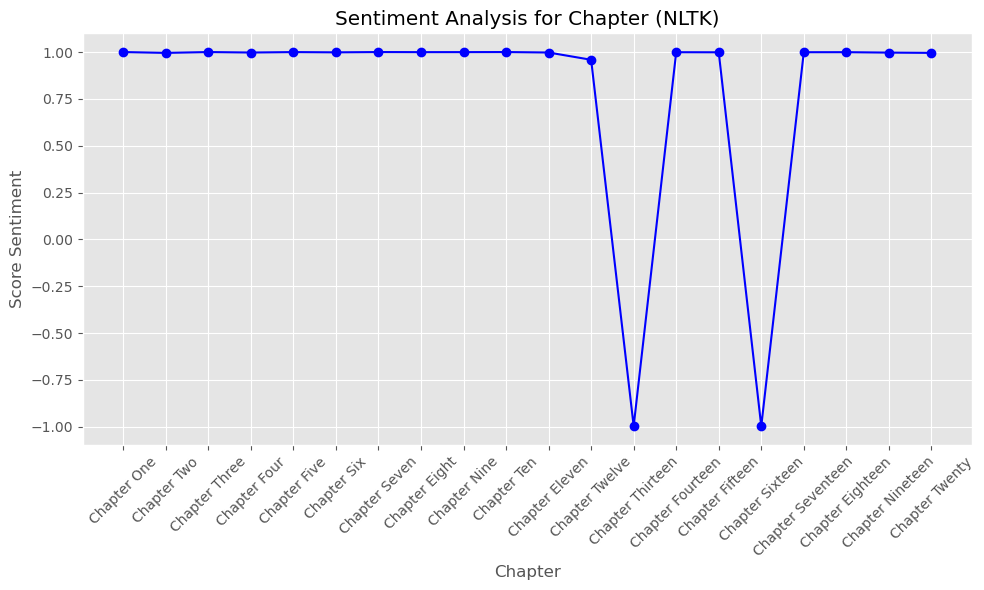
\includegraphics[width=0.5\textwidth]{graph/nltksent.png}
    \caption{Sentiment Analysis with NLTK}
    \label{fig:example}
\end{figure}


RoBERTa is a more sophisticated deep-learning approach: it performs a more accurate sentiment analysis, it can understand context and sarcasm and is able to capture nuanced sentiments. This model made it possible to accomplish a more accurate analysis, but its computational cost is quite heavy: I was able to successfully run it only after splitting the text into chunks, and it still was not successful every time.
The graph shows a more realistic development of the plot. It’s interesting to notice that the whole books has a negative score and the last chapter is slightly more positive than the first one. The lowest score is the one for chapter twelve, where Esther receives shock treatment the first time, while the highest is in chapter seventeen, when she gets moved to a ward for women closer to release. The positive trend from chapter twelve to fifteen doesn’t represent the downward spiral the Esther’s mental state follows.

\begin{figure}[h]
    \centering
    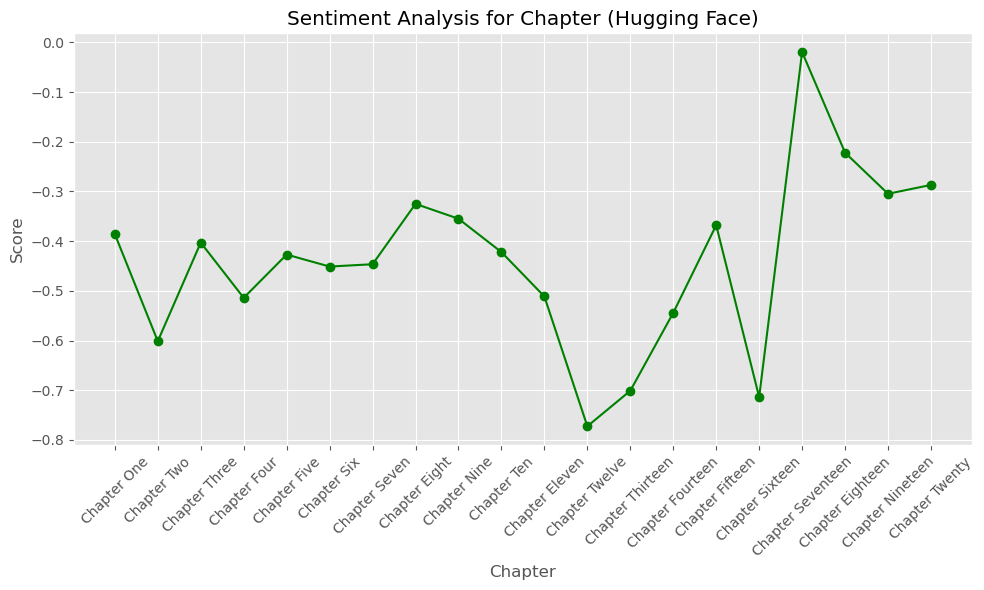
\includegraphics[width=0.5\textwidth]{graph/hugsent.png}
    \caption{Sentiment Analysis with RoBERTa}
    \label{fig:example}
\end{figure}

\section{Computational linguistic analysis}

\subsection{Thematic Analysis}

Another way that could be useful to analyze the Esther’s mental health is Topic Modeling. Latent Dirichlet Allocation (LDA) is a generative probabilistic model that assumes each topic is a mixture over an underlying set of words, and each document is a mixture of over a set of topic probabilities. I coded a script that shows one topic for chapter, and one that shows the most frequent topics in the whole book, so that it was possible to use the pyLDAvis visualization package. The first is useful, as it shows how the themes changes chronologically, while the latter, thanks to its interactivity, provides better understanding of individual topics and the relationships between them. 
The topics got for each chapters show successfully the keywords to summarize the plot: the most relevant characters are shown when they influence Esther’s life, and together with the locations mentioned, it is possible to understand what is happening in the story.
The graph shown through pyLDAvis, portraits ten topics: none of those are intersecting each other, meaning these topic are not conceptually similar. Adjusting the lambda value close to zero highlights the words who are more unique to a specific topic, doing so gives a different perspective on what defines each topic: the main topics relate to love, mental hospitalization and religion.

\subsection{The Language of Depression}
An N-gram is a sequence of n words found in the text, to analyze common phrases and word pairings. To perform these tasks, the text was tokenized first, then I decided to form bi-grams and tri-grams, so i plotted two graphs that showed the 20 most frequent.
The Word Frequency approach calculates how often each word appears in the text, highlighting key terms and ideas. The tokenized text is cleaned: i removed stop words to focus on more meaningful terms. The frequency of each word is calculated, then the most common words are selected and plotted, allowing a clear view of dominant vocabulary. This can show key ideas, repeated themes, and the character focus in the story.
Through these analyses, I got interesting information about the character, which I am going to discuss later, and the most frequent vocabulary.
Mohammed Al-Mosaiwi analyzed the “language of depression” through computerized text analysis methods and what he discovered can also be found in this statistical analysis. 
Through the grep command in the command line, I was able to find where the words that interested me were mentioned, so i could find them in context. A significant use of the first person pronoun is part of depression language, but since this book is written from Esther’s point of view, it wouldn’t be correct to simply count how many “I”, “myself” and “me” there are, but it’s still interesting to point out that most of the verbs in the N-gram analysis have Esther has a subject.  The style is more relevant characteristic to look at, since it is how people decide to express themselves. People that suffer from depression use absolutist words, mirroring a black and white view of the word (\citename{Rude \textit{et al.}}); this is the case for Esther as well, as shown by the tri-gram graph (“didn’t say anything”, “knew perfectly well”, “never get anywhere”, …).

\begin{figure}[h]
    \centering
    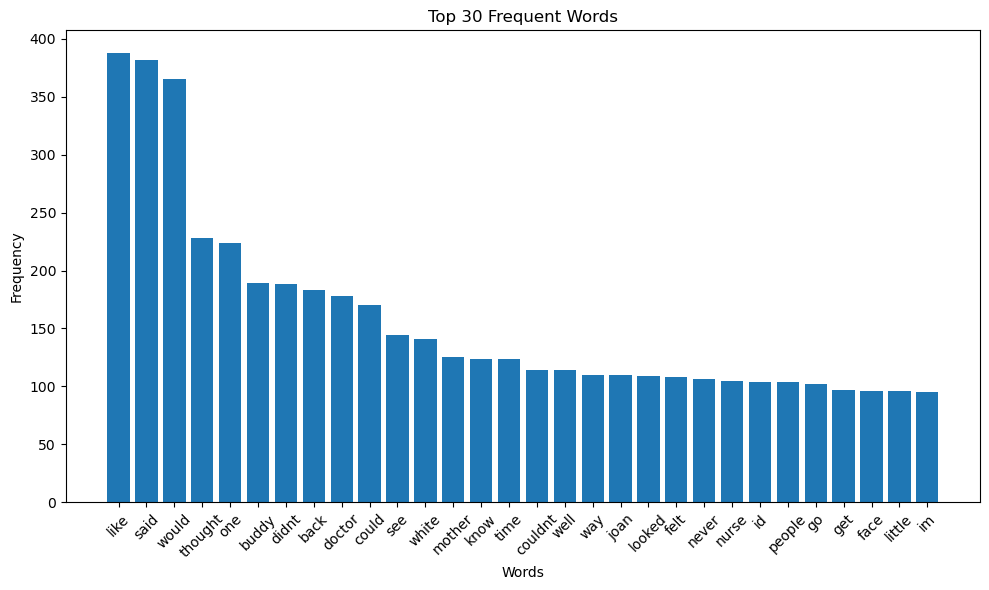
\includegraphics[width=0.5\textwidth]{graph/freqlist.png}
    \caption{Most frequent words}
    \label{fig:example}
\end{figure}

\begin{figure}[h]
    \centering
    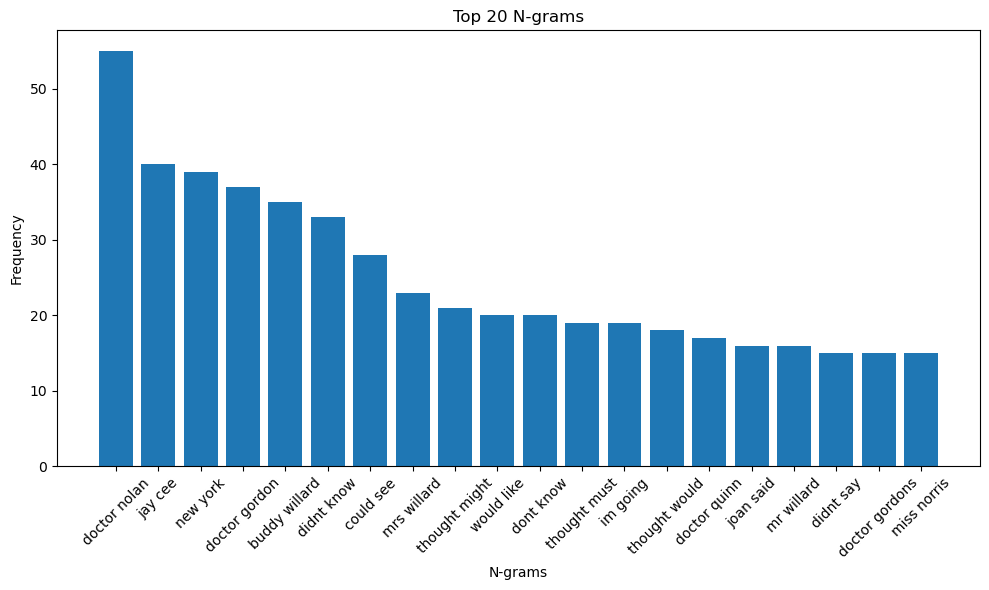
\includegraphics[width=0.5\textwidth]{graph/2grams.png}
    \caption{Most frequent Bi-grams}
    \label{fig:example}
\end{figure}

\begin{figure}[h]
    \centering
    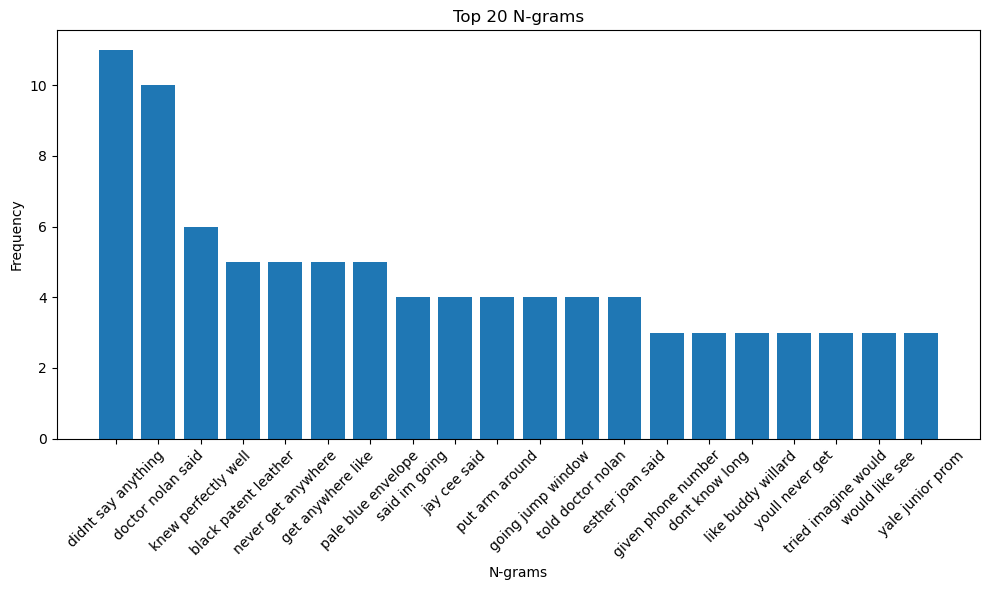
\includegraphics[width=0.5\textwidth]{graph/3grams.png}
    \caption{Most frequent Tri-grams}
    \label{fig:example}
\end{figure}

\subsection{Wordcloud and Character Network}

The word cloud presents the most frequent words in the text, emphasizing commonly occurring words visually.
Through this device, it is possible to see more absolutist words (“never”, “always”), but also the word “thought”, can be interpreted as another sign of depression: ruminating, the act of dwelling on personal problems. It is also possible to see how relevant Esther’s mental hospitalization is, compared to the rest of the plot, and how much Buddy Willard and Esther’s mom are present in the protagonist’s mind. Also, “Buddy” is sixth most frequent word, making him the most mentioned character. In the Character Network, he is also the closest to Esther.

\begin{figure}[h]
    \centering
    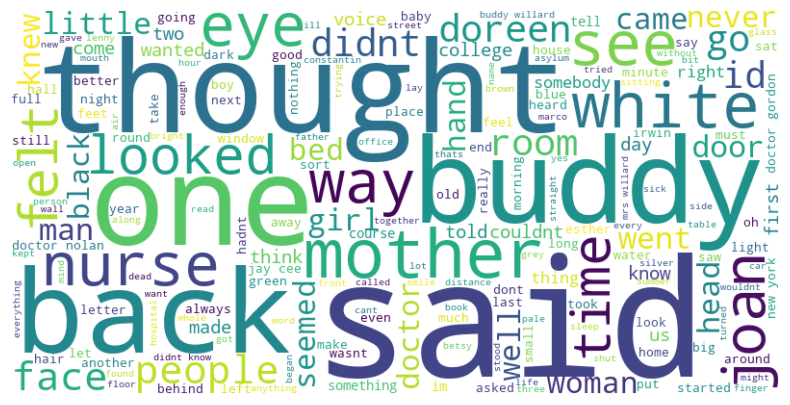
\includegraphics[width=0.5\textwidth]{graph/wordcloud.png}
    \caption{Wordcloud}
    \label{fig:example}
\end{figure}

The Character Network visualizes relationships between key figures in The Bell Jar by representing them as nodes in a graph, with edges (connections) between them based on their co-occurrences. After parsing the data and deciding which characters would have been relevant, a co-occurrence analysis is performed then, through NetworkX, I constructed the network: nodes represent characters, and weighted edges are added between nodes based on their co-occurrence frequency, indicating the strength of their interaction.
Unfortunately, the Character Network gives a imprecise visualization: it portrays Miss Greenwood, or Esther’s mother, very distant from her, even though she plays an important role in the plot. This is because she is rarely mentioned by name, but since “mother” is a common word,and Buddy's mother is mentioned multiple times, that would also bring to an incorrect results.

\begin{figure}[h]
    \centering
    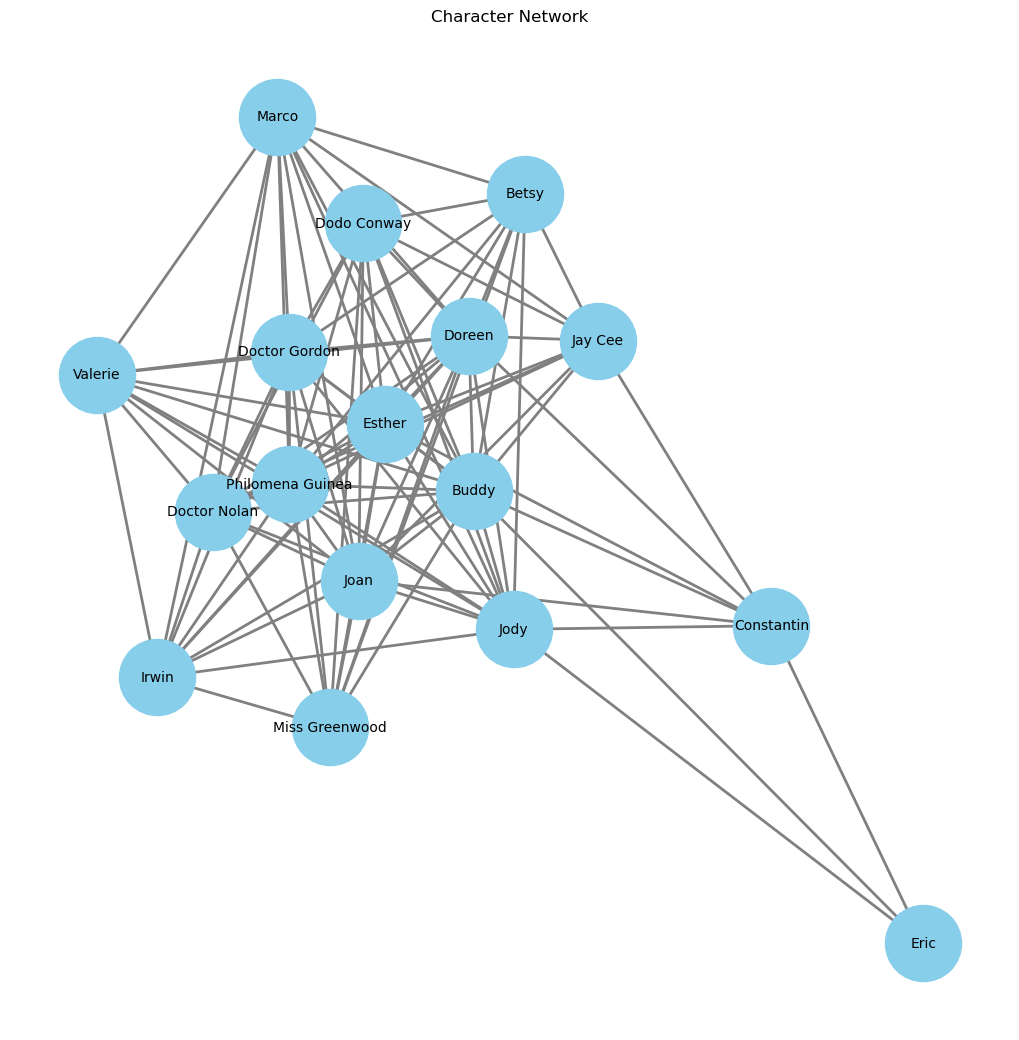
\includegraphics[width=0.5\textwidth]{graph/charanet.png}
    \caption{Character Network}
    \label{fig:example}
\end{figure}

\section{Conclusion}
This project provided a multi-layered analysis of The Bell Jar by using natural language processing to delve into the themes, style, and emotional tone of Sylvia Plath's work. 
Comparing two Sentiment Analysis models brought me two completely different result: the Vader model doesn’t perform well on texts like this, but even though RoBERTa has a better performance, i think it could be improved, maybe by not using a pre-trained model, but training one for the specific task of detecting mental illnesses.
The linguistic analysis brought interesting results that could be used in a deeper literary analysis, and as a new method that provides a fresh perspective: the structural and statistical approach can highlight details a reader maybe does not get. Future work might involve cross-genre comparisons or an exploration of the author’s other works to further contextualize what was revealed in this analysis.

\section{Work organization}
To do this project alone, I learned more about the tasks i wanted to work on through different YouTube tutorials. ChatGpt was used, in particular to fix the issues I found while using the RoBERTa model for sentiment analysis. I worked on Pycharm and uploaded the project on GitHub once I was finished, by pushing my existing repository through the command line.

\begin{thebibliography}{}

\bibitem[\protect\citename{Bird, Klein, and Loper}2024]{NLTK:24}
Bird, S., Klein, E., and Loper, E.
\newblock 2024.
\newblock {\em Natural Language Toolkit (NLTK)}.
\newblock Retrieved from \url{https://www.nltk.org}.

\bibitem[\protect\citename{Pedregosa \textit{et al.}}2024]{ScikitLearn:24}
Pedregosa, F., Varoquaux, G., Gramfort, A., \textit{et al.}
\newblock 2024.
\newblock {\em Scikit-Learn: Machine Learning in Python}.
\newblock Retrieved from \url{https://scikit-learn.org/stable/}.

\bibitem[\protect\citename{Bird}2024]{NLTKConcordance:24}
Bird, S.
\newblock 2024.
\newblock {\em Concordance with NLTK}.
\newblock Retrieved from \url{https://www.nltk.org/howto/concordance.html}.

\bibitem[\protect\citename{Onu}2023]{Onu:23}
Onu, B.
\newblock 2023.
\newblock VADER vs. RoBERTa: A Comparison of Sentiment Analysis Models.

\bibitem[\protect\citename{Mueller}2024]{WordCloud:24}
Mueller, A.
\newblock 2024.
\newblock {\em WordCloud Python Package}.
\newblock Retrieved from \url{https://pypi.org/project/wordcloud/}.

\bibitem[\protect\citename{Hagberg \textit{et al.}}2024]{NetworkX:24}
Hagberg, A., Schult, D., and Swart, P.
\newblock 2024.
\newblock {\em NetworkX Reference Documentation}.
\newblock Retrieved from \url{https://networkx.org/documentation/stable/reference/introduction.html}.

\bibitem[\protect\citename{Shubham}2024]{Shubham:24}
Shubham, B.
\newblock 2024.
\newblock End-to-End Topic Modeling in Python: Latent Dirichlet Allocation (LDA).

\bibitem[\protect\citename{Thompson \textit{et al.}}2024]{Thompson:24}
Thompson, K., Mazidi, M., and Johnson, J.
\newblock 2024.
\newblock {\em Machine Learning Analysis of Depression Language Patterns}.
\newblock Retrieved from \url{https://www.ncbi.nlm.nih.gov/pmc/articles/PMC9331452/}.

\bibitem[\protect\citename{Skorczewski}2006]{Skorczewski:06}
Skorczewski, D.
\newblock 2006.
\newblock Sylvia Plath’s Use of Figurative Language in The Bell Jar.
\newblock {\em Plath Profiles}, 1(1):47--50.
\newblock Retrieved from \url{https://scholarworks.iu.edu/journals/index.php/plath/article/view/4714/4350}.

\bibitem[\protect\citename{Research Blog}2018]{Reading:18}
University of Reading.
\newblock 2018.
\newblock People with Depression Use Language Differently: Here’s How to Spot It.

\bibitem[\protect\citename{Rude \textit{et al.}}2016]{Rude:16}
Rude, S., Gortner, E., and Pennebaker, J.
\newblock 2016.
\newblock Language Use in Depressive States.
\newblock {\em Journal of Language and Social Psychology}, 36(2):135--142.
\newblock Retrieved from \url{https://journals.sagepub.com/doi/full/10.1177/0261927X15589186}.

\end{thebibliography}

\end{document}
